% Appendix A

\chapter{Appendix A Gantt Details} % Main appendix title

\label{AppendixA} % For referencing this appendix elsewhere, use \ref{AppendixA}


Figure \ref{fig:gantt_complete} presents a comprehensive Gantt chart showing all project sub-tasks and their corresponding columns. The chart reveals a more granular task breakdown compared to the \gls{WBS} deliverables. Notably, the design and implementation phases demonstrate an approach of concurrent task execution. For instance, the actual task realization begins simultaneously with the process of studying tools and potential solutions. This deliberate scheduling strategy allows for parallel exploration and development, with the study phase specifically allocated time for focused research and evaluation. The variance column was omitted from the visual representation to maintain image clarity, as its details were already comprehensively addressed in the main document. Similarly, the baseline, positioned at the project's inception, was excluded to prevent unnecessary visual complexity.

\begin{figure}
    \centering
    \frame{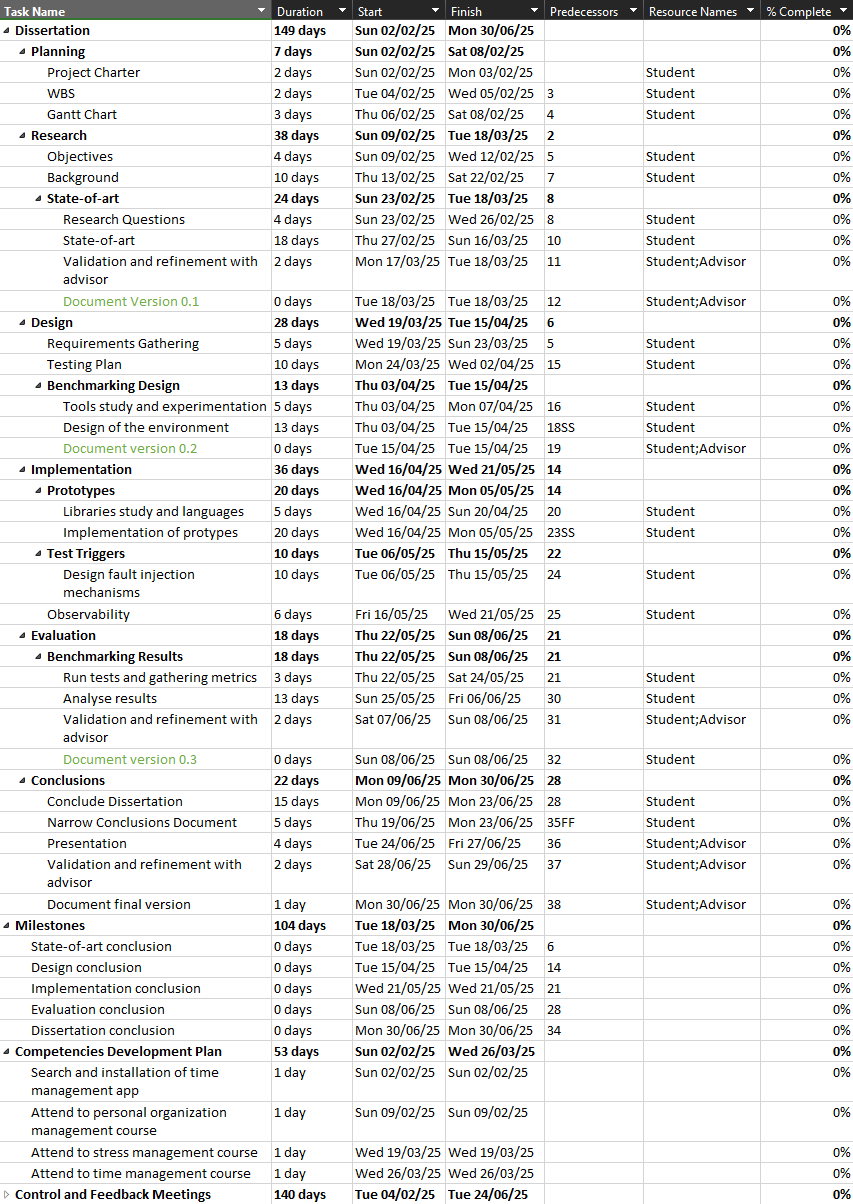
\includegraphics[width=\linewidth]{appendices/assets/gantt_complete.png}}
    \caption{Complete demonstration of the Gantt}
    \label{fig:gantt_complete}
\end{figure}